In this chapter, we propose a generic theory for active nematic deformable surfaces. The state of the system is given by the shape of the surface, the nematic tensor on the surface, and the surface density of cytoskeletal materials, which evolves as a result of local area changes and of turnover. Accounting for density allows us to describe interfacial active gels such as the actomyosin cytoskeleton, which experiences very large density variations often coupled to changes of nematic order. This framework can be very easily adapted to more conventional liquid crystal surface models, where density does not play such an important role, and instead the surface is often considered to be locally inextensible. Such a model is developed in Chapter~\ref{chap_9} and is pertinent for instance to active nematic gels deforming on lipid vesicles. Our derivation is based on the variational framework for active surfaces proposed in \cite{torres2019}. We start by describing the state variables of the model, followed by the process variables describing their evolution. We then resort to Onsager's variational formalism to systematically derive the Euler-Lagrange equations of the model. As described in previous chapters, the variational formulation is useful for coupling surface flow with other relevant mechanical and chemical effects as well as for numerical finite element implementations. At the core of the variational framework is the Lagrangian of the system formulated as the sum of  1) a dissipation potential encoding the passive and unrecoverable energetic cost of changing the state of the system, 2) the rate-of-change of the free-energy potential describing the release rate or reversible work, 3) a power potential capturing the active power input and 4) the work performed by Lagrange multipliers to subject the system to mechanical constraints. The Lagrangian functional is minimized with respect to the process variables and maximized with respect to the Lagrange multipliers to derive the  Euler-Lagrange equations in a thermodynamically consistent manner. In this model, in the absence of active power input, the free-energy is by construction a Lyapunov function of the dissipative dynamics.  For an extensible surface, the model is complemented by a mass balance equation describing turnover.  

The outline of this chapter is as follows. In Section~\ref{sec4_2_1}, we start by introducing our notations and the differential geometry required to describe the state and process variables of a nematic surface. In Section~\ref{sec4_2_2}, we derive the  strong form of a thermodynamically consistent nematic active deformable surface following Onsager's variational formalism. Finally, in Section~\ref{sec4_2_4}, we summarize our results.

\section{Kinematics of nematic surfaces} \label{sec4_2_1} 

\subsection{Differential geometry and covariant derivatives}

We describe the dynamics of a two-dimensional continuum $A$ in $\mathbb{R}^3$ using a time-dependent parametrization of the surface $\bm{x}=\bm{\phi}(\bm{\xi},t)$ from a reference domain $\bar{A}$ with coordinates $\bm{\xi}=\{\xi^1, \xi^2$\}  in $\mathbb{R}^2$, see Fig.~\ref{fig_7.1}. This time-dependent map can be interpreted as a Lagrangian parametrization, i.e.~for a fixed $\bm{\xi}$, $\bm{\phi}(\bm{\xi},t)$ tracks the trajectory of a material particle. At any instant $t$ and coordinate $\bm{\xi}$, the natural or convected basis vectors of the tangent plane to $A$ are given by $\bm{e}_1 = \partial_{1} \bm{\phi}$ and $\bm{e}_2 = \partial_{2} \bm{\phi}$, where $\partial_a = \partial / \partial \xi^a$. In general, these basis vectors are neither of unit length nor orthogonal. The  normal vector to $A$ at $\bm{x}=\bm{\phi}(\bm{\xi})$ is given by $\bm{N} = (\bm{e}_1 \times \bm{e}_2)/\left|\bm{e}_1 \times \bm{e}_2 \right|$. Here and in the following, we use upper-case letters to denote three-dimensional tensors and lower-case letters for tensors tangent to $A$, i.e.~without a normal component. 
\begin{figure}[h!]
	\centering
	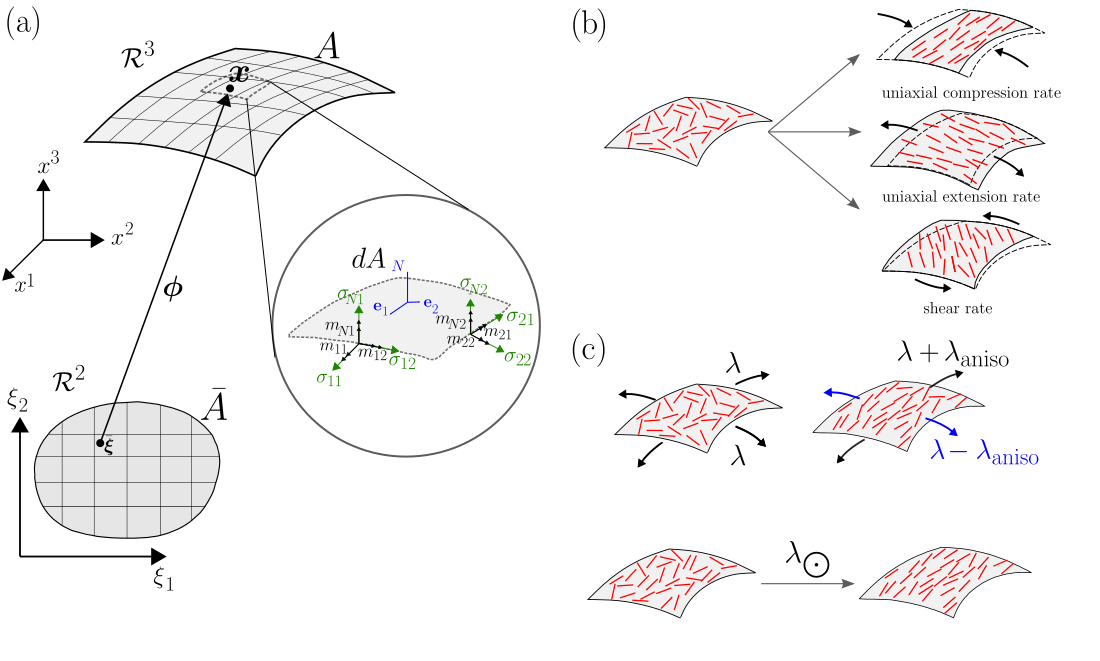
\includegraphics[width=1\textwidth]{chap_7_fig_1.pdf}
	\caption{(a) Illustration of the surface parametrization, with the induced local basis of the tangent space given by  $\bm{e}_1$ and $\bm{e}_2$, and the normal unit vector $\bm{N}$. The inset shows the different stress components, including the in-plane stress $\bm{\sigma}$, the out-of-plane stress $\bm{\sigma}_N$, the in-plane moment $\bm{m}$ and the out-of-plane moment $\bm{m}_N$. (b) A compression (extension) in the local area results in an emergent nematic order with molecular aligned on average perpendicular (along) to the principal direction of the rate of deformation tensor $\bm{d}$. A shear in the local area  due to traceless $\bm{d}^{\rm dev}$ tends to align fibers clockwise or counter-clockwise depending on the direction in which the differential area element distorts. (c) $\lambda \bm{g}$ characterizes the base value of the emergent isotropic active stress per unit volume resulting from the action of actin bundling proteins in an isotropic network.  $\lambda_{\rm aniso} \bm{q}$ characterizes the base value of emergent  anisotropic active stress per unit volume resulting from the action of actin bundling proteins in an anisotropic network along ($\lambda_{\rm aniso}>0$) or perpendicular ($\lambda_{\rm aniso}<0$) the average molecular orientation $\bm{n}$.  $\lambda_{\bigodot}\bm{q}$ characterizes the basal active torque per unit volume exerted by the actin bundling proteins resulting in filament rotational movement.}
	\label{fig_7.1}
\end{figure} 
We define the dual basis $\{\bm{e}^1,\bm{e}^2\}$, satisfying the conditions
\begin{equation} \label{2_II}
	\bm{e}^a \cdot \bm{e}_b = \delta^a_b,
\end{equation}
where here $\cdot$ stands for the scalar product in Euclidean space. 
Given a tangent vector $\bm{v}$, we can represent it in terms of the natural and dual basis, $\bm{v}=v^a\bm{e}_a=v_a\bm{e}^a$. We call $v^a$ the contravariant components of $\bm{v}$ and $v_a$ the covariant components of $\bm{v}$. Given that $\bm{v}$ is also embedded in Euclidean space, we can represent it as $\bm{v}=v^\alpha \bm{E}_\alpha$ where the vectors $\bm{E}_\alpha$, $\alpha=1,2,3$ form an orthonormal basis of Euclidean space. In the following, we use Latin indices, running from $1$ to $2$, for components in the tangent plane and Greek indices, running from $1$ to $3$, for components in Euclidean space. 

The metric tensor $\bm{g}$ can be used to compute the scalar product of vectors on $A$: given two tangent vectors $\bm{v} = v^a \bm{e}_a$ and  $\bm{w} = w^b \bm{e}_b$, their scalar product is $\bm{v}\cdot\bm{w}=\bm{g}(\bm{v},\bm{w})=g_{ab} v^a w^a$. Since $\bm{v}\cdot\bm{w}$ is also defined in Euclidean space, this equivalence can be used to find the components of $\bm{g}$ in the basis $\{\bm{e}^1,\bm{e}^2\}$:
\begin{equation} \label{eq::metric}
	g_{ab} = \bm{e}_a \cdot \bm{e}_b.
\end{equation}
The inverse of $\bm{g}$, $\bm{g}^{-1}=g^{ab}\bm{e}_a\otimes\bm{e}_b$, satisfies $g^{ac}g_{cb} = \delta^a_{~b}$. We note that $\bm{e}^a$ and $\bm{e}_a$ satisfy
\begin{equation} \label{2_II}
	\bm{e}^a = g^{ab}\bm{e}_b,\qquad \bm{e}_a = g_{ab}\bm{e}^b.
\end{equation}
Similarly, the contravariant and covariant components of a vector satisfy 
\begin{equation}
	v_a = g_{ab} v^b,\qquad v^a = g^{ab} v_b. 
\end{equation}
These operations are referred to as lowering and raising an index.

The curvature tensor on $A$, $\bm{k}$, measuring how much the surface deviates from a plane, can be defined through derivatives of $\bm{N}$. In particular $k_{ab}$ measures the rate of change of $\bm{N}$ along $\bm{e}_a$ in the direction of $\bm{e}_b$,
\begin{equation} \label{3_II}
	k_{ab} = \partial_b \bm{N} \cdot \bm{e}_a = -\bm{N} \cdot  \partial_a  \partial_b \bm{\phi},
\end{equation}
where to get to the last expression we have used the product rule and that $\bm{N} \cdot \bm{e}_a=0$.
The antisymmetric tensor $\bm{\epsilon}$, satisfying $\epsilon_{ab}=-\epsilon_{ba}$ and $\epsilon_a{}^c \epsilon^b{}_c=\delta_a^b$ has components
\begin{equation} \label{4_II}
	\epsilon_{ab} = \bm{N} \cdot (\bm{e}_a \times \bm{e}_b).
\end{equation}

To measure derivatives of tensors on $A$, we use the covariant derivative $\nabla$, which accounts for the fact that both the components of a tensor and the basis vectors vary along the curvilinear coordinates. For a vector, $\nabla\bm{v}$ has components
\begin{equation} \label{6_II}
	\nabla_b v^a = \partial_b v^a + \Gamma^a{}_{bc} v^c.
\end{equation}
where $\Gamma^c_{~ ab}$ are the Christoffel symbols of the basis $\{\bm{e}_1,\bm{e}_2\}$. These quantities  measure the rate of change of $\bm{e}_a$ along $\bm{e}_b$ in the direction of $\bm{e}^c$,
\begin{equation} \label{8_II}
	\Gamma^c_{~ ab} = \bm{e}^c\cdot \partial_b \bm{e}_a=\bm{e}^c\cdot \partial_b \partial_a \bm{\phi},
\end{equation}
and can be expressed intrinsically in terms of derivatives of the metric tensor alone \cite{Do_Carmo2016-kq}.
Given that $\partial_b \partial_a \bm{\phi}=\partial_a \partial_b \bm{\phi}$, we have $\Gamma^c_{~ ab}= \Gamma^c_{~ba}$. The covariant derivative
$\nabla\bm{v}$ can be defined intrinsically to the surface $A$ seen as a Riemannian manifold without reference to the embedding Euclidean space. It can also be related to the  usual gradient in $\mathbb{R}^3$ by
\begin{equation}\label{cov_der}
	\nabla \bm{v} = \mathbb{P}\,\nabla^{\rm 3D} \bm{v}\,\mathbb{P}
\end{equation}
where $\mathbb{P}=\bm{e}^a\otimes\bm{e}_a$ is the projector operator on the surface and $\otimes$ is the tensor product (see Appendix~\ref{velocity_gradient}). The projector on the right restricts the derivative to the plane, whereas the projector on the left ensures that the result is tangent to $A$. Computing $\nabla^{\rm 3D}$ requires extending the field $\bm{v}$ outside of $A$, but it can be shown that the result is independent of the extension because of the action of the right projector. 
The covariant derivative of $\bm{v}$ written in terms of its covariant components is given by
\begin{equation} \label{6_II_b}
	\nabla_b v_a = \partial_b v_a - \Gamma^c_{ab} v_c.
\end{equation}
For a generic tensor $\bm{T}$ described with $m$ contravariant and $n$ covariant components, the definition of the covariant derivative is
\begin{align} \label{7_II}
	\nabla_c T^{a_1\dots a_m}_{~ \, \, \, \, \, \, \, \, \, \, \, \, \, \, \, \,   b_1 \dots b_n} =  {}&  \partial_c T^{a_1 \dots a_m}_{~ \, \, \, \, \, \, \, \, \, \, \, \, \, \, \, \, b_1 \dots b_n}  + \Gamma^{a_1}_{cd} T^{d\dots a_m}_{~ \, \, \, \, \, \, \, \, \, \, \, \, \, \, \, \,   b_1 \dots b_n} + \Gamma^{a_2}_{cd} T^{a_1 d\dots a_m}_{~ \, \, \, \, \, \, \, \, \, \, \, \, \, \, \, \,   b_1 \dots b_n} + \left(\text{all upper indices}\right)   \nonumber\\ & - \Gamma^d_{c b_1} T^{a_1 \dots a_m}_{~ \, \, \, \, \, \, \, \, \, \, \, \, \, \, \, \, d \dots b_n} -  \Gamma^d_{c b_2} T^{a_1 \dots a_m}_{~ \, \, \, \, \, \, \, \, \, \, \, \, \, \, \, \, b_1 d \dots b_n}  - \left(\text{all lower indices}\right),
\end{align}
Notably, 
\begin{align} \label{10_II}
	\nabla\bm{g} = \nabla\bm{g}^{-1} = \nabla\bm{\epsilon} = \bm{0},
\end{align}
We can extend the notion of the covariant derivative to 3D tensors defined over $A$. For instance, given a vector $\bm{V}$,
\begin{equation}\label{cov_derV}
	\nabla \bm{V} = \nabla^{\rm 3D} \bm{V}\,\mathbb{P},
\end{equation}
Note that here, the right projector is used again to restrict the computation to variations along the tangent plane, whereas the left projector is absent given that we want to know how the vector is changing in Euclidean space. This is a $3\times2$ tensor with first component in Euclidean space and second component tangent to $A$. Eq.~\eqref{cov_derV} can be rewritten in terms of the in-plane  and normal components of $\bm{V} = \bm{v} + v_N \bm{N}$ as
\begin{equation}
	\label{eq::velgrad}
	\nabla \bm{V}= \left(\nabla_b v^a+v_n k_b{}^a \right) \bm{e}_a \otimes \bm{e}^b + \left(\nabla_a v_n - k_{ab} v^b \right) \bm{N} \otimes \bm{e}^a.
\end{equation}
See Appendix~\ref{velocity_gradient} for a derivation. 

\subsection{Velocity, rate of deformation, and spin}

The velocity field is defined as
\begin{equation} \label{14_II}
	\bm{V} = \partial_t \bm{\phi}(\bm{\xi},t) = \bm{v} + v_N \bm{N},
\end{equation}
where the normal velocity $v_N$ characterizes the rate of change of the shape of $A$ and $\bm{v}$ describes the in-plane flow. The velocity gradient is given by the covariant derivative of $\bm{V}$ defined by Eq.~\eqref{eq::velgrad}. On a plane, we have seen previously in this thesis that we can split the velocity gradient into its symmetric and antisymmetric parts
\begin{equation}\label{qwe}
	\nabla\bm{v} = \bm{d} + \bm{w}
\end{equation}
where $\bm{d}$ ($=\bm{d}^T$), the rate-of-deformation tensor, characterizes the strain rate and $\bm{w}$ ($=-\bm{w}^T$) the spin tensor, characterizes the local rotation generated by the flow. We seek a similar decomposition for $\nabla\bm{V}$. We first note that the rate-of-deformation tensor admits the following geometric definition \cite{marsden1994}
\begin{equation}\label{eq6:lie-der}
	\bm{d}=\frac{1}{2}\mathcal{L}_{\bm{V}}\bm{g},
\end{equation}
where $\mathcal{L}_{\bm{V}}\bm{g}$ is the Lie derivative of $\bm{g}$. This quantity measures the rate of change of the metric tensor $\bm{g}$ as seen by an observer that deforms with the flow generated by $\bm{V}$. The Lie derivative satisfies the product rule, which allows us to compute the Lie derivative of the inverse of the metric. Because $0 = \mathcal{L}_{\bm{V}} \delta^a_b = \mathcal{L}_{\bm{V}}(g^{ac}g_{cb}) = g_{cb}\mathcal{L}_{\bm{V}}g^{ac} + g^{ac}\mathcal{L}_{\bm{V}}g_{cb} = g_{cb}\mathcal{L}_{\bm{V}}g^{ac} + 2 g^{ac}d_{cb}$, we conclude that $\mathcal{L}_{\bm{V}}g^{ab} = -2 d^{ab}$, or tensorially 
\begin{equation}\label{eq6:lie-der_}
	\bm{d}= - \frac{1}{2}\mathcal{L}_{\bm{V}}\bm{g}^{-1}.
\end{equation}

Because our parametrization is Lagrangian, its components are given in the natural convected basis of the surface by $\mathcal{L}_{\bm{V}}g_{ab} = \partial_t\left(\bm{e}_a\cdot\bm{e}_b\right)=\bm{e}_a\cdot\partial_b\bm{V} + \bm{e}_b\cdot\partial_a\bm{V}$, which can be written in terms of $\nabla\bm{V}$ as
\begin{equation}
	\label{eq6:d}
	\bm{d} = {\rm sym}\left(\mathbb{P}\,\nabla \bm{V}\right)= \frac{1}{2}\left[\nabla \bm{v} + \left(\nabla\bm{v}\right)^T\right] + v_N \bm{k}.
\end{equation}
Since $\bm{g}$ determines the length and angle between vectors on $A$, $\mathcal{L}_{\bm{V}}\bm{g}$ characterizes the rate at which objects deform on the surface \cite{torres2017}. For instance, the trace of $\bm{d}$ characterizes the rate of change of an infinitesimal area
\begin{equation}\label{eq6:dSdt}
	\frac{1}{dS}\dfrac{d}{dt}dS = \textup{tr}\bm{d} = d_{ab}g^{ab} = \nabla \cdot \bm{v} + v_N H,
\end{equation}
where $\nabla \cdot \bm{v}=\nabla_a v^a$ is the divergence of the in-plane velocity and $H=\textup{tr}(\bm{k})$ is the total curvature (twice the mean curvature).

To find an expression analogous  to Eq.~(\ref{qwe}) in the surface setting, we examine the structure of $\nabla \bm{V} - \bm{d}$, which should yield the generalization of the spin tensor. Combining Eqs.~(\ref{eq::velgrad}) and (\ref{eq6:d}), it follows that this difference can be uniquely expressed in terms of a three-dimensional spin tensor $\bm{W}$, satisfying $\bm{W}^T=-\bm{W}$, as
\begin{equation}
	\nabla \bm{V} - \bm{d} = \bm{W} \mathbb{P},
\end{equation}
where
\begin{equation}
	\bm{W} = \frac{1}{2}\left(\nabla_b v_a - \nabla_a v_b\right) \bm{e}^a\otimes \bm{e}^b + \left(\nabla_a v_N - k_{ab} v^b \right) \left(\bm{N} \otimes \bm{e}^a -  \bm{e}^a\otimes \bm{N}\right).
\end{equation}
The first component arises from local in-plane rotations rates and corresponds to the previously considered spin tensor in the flat case. The second component represents the local rotation rate of the surface tangent plane in $\mathbb{R}^3$. Thus, the velocity gradient can be decomposed into the rate of deformation tensor and the projection onto the tangent plane to $A$ of a three-dimensional spin tensor
\begin{equation}
	\nabla \bm{V} = \bm{d} + \bm{W} \mathbb{P}.
\end{equation}
One can also define the spin vector, $\bm{\Omega} = \bm{W}^\star$, the Hodge-dual of $\bm{W}$ in $\mathbb{R}^3$, whose Cartesian components are
\begin{equation} \label{omega_alpha}
	\Omega^\alpha = \mathcal{E}^{\alpha\beta\gamma} W_{\beta\gamma} = \omega_a  e^{a\alpha} + \omega_N N^{\alpha}.
\end{equation}
where $\bm{\mathcal{E}}$ is the 3D Levi-Civita tensor and where
\begin{align}
	\bm{\omega} &= \bm{\epsilon}\left(\nabla v_N - \bm{k}\bm{v}\right),\label{eq6:omega}\\
	\omega_N &= \frac{1}{2} \epsilon^{ab} \nabla_b v_a. \label{eq6:omegaN}
\end{align}
In Eq.~(\ref{omega_alpha}), $e^{a\alpha}$ denotes the $\alpha$-th Cartesian component of tangent vector $\bm{e}^a$. The spin tensor can be recovered from the spin vector from $W^{\alpha\beta} = \mathcal{E}^{\alpha\beta\gamma}\Omega^\gamma$. 

The covariant derivative of the spin vector, quantifying the gradients of rotation rate, is given by
\begin{equation}
	\bm{\mathcal{Z}} =\nabla \bm{\Omega}  = \zeta^a{}_b\bm{e}_a \otimes \bm{e}^b + \zeta_{na} \bm{N} \otimes \bm{e}^a,
\end{equation}
where
\begin{align}
	\bm{\zeta} &= \nabla \bm{\omega}+\omega_N\bm{k},\label{eq6:xi}\\
	\bm{\zeta}_N &= \nabla \omega_N-\bm{k}\bm{\omega}\label{eq6:xiN}.
\end{align}
The Lie derivative of the curvature tensor (with covariant indices) can be written in terms of $\bm{\zeta}$ and $\bm{d}$ as
\begin{align} \label{26_II}
	\mathcal{L}_{\bm{V}} \bm{k}  = & -\frac{1}{2} \left(\bm{\zeta} +\bm{\zeta}^T\right)+ \frac{1}{2}\left(\bm{k}\,\bm{d} +\bm{d}\,\bm{k}\right),
\end{align}
see Appendix~\ref{curvature_tensor}.
Similarly, the rate of change of the Christoffel symbols in the convected basis satisfies
\begin{equation}\label{25_II}
	 \zeta_{Nc} = \frac{1}{2}\partial_t\Gamma^a_{bc} \epsilon_a^{~b} .
\end{equation}
%see Appendix~\ref{christoff_symbols}.

\subsection{Nematic order}


Another state variable characterizing the system is the nematic order tensor $\bm{q}$, which measures orientational order tangentilly to $A$. Mathematically, it is expressed as
\begin{equation} \label{27_II}
	\bm{q} = S\left(\bm{n}\otimes\bm{n} - \frac{1}{2}\bm{g}\right),
\end{equation}
where $\bm{n}$, a vector, represents the local director field and $S=\sqrt{2q_{ab}q^{ab}}$, the nematic order parameter, represents the strength of alignment about $\bm{n}$. The nematic tensor is both symmetric, $\bm{q} = \bm{q}^T$, and traceless $\textup{tr}\bm{q}=0$. We now need to define an objective rate for $\bm{q}$. In 2D, we have used the Jaumann derivative,
\begin{equation}\label{eq6:Lie-der-q}
	\widehat{\bm{q}} = \partial_t\bm{q} + \bm{v}\cdot\nabla\bm{q} + \bm{q}\bm{w} + \bm{w}\bm{q}.
\end{equation}
We cannot translate this equation directly to the case of a nematic field evolving on a deforming surface since each of the terms do not have a clear translation. To make sense of the Jaumann derivative in our more general situation, we note that objective rates of tensors can be expressed geometrically in terms of Lie derivatives of such tensors \cite{marsden1994}. Indeed, the Jaumann derivative can be expressed as the average of the Lie derivatives of the covariant and of the contravariant forms of the nematic tensor 
\begin{align}\label{jaum_1}
	\widehat{q}^{ab}  = \frac{1}{2}\left(\mathcal{L}_{\bm{V}} q^{ab}  +  g^{ae}g^{bf} \mathcal{L}_{\bm{V}} q_{ef}  \right). 
\end{align}
This definition can be naturally extended to covariant and mixed tensors as
\begin{align}
	\widehat{q}_{ab}  = \frac{1}{2}\left(g_{ae}g_{bf} \mathcal{L}_{\bm{V}} q^{ef}  + \mathcal{L}_{\bm{V}} q_{ab}  \right), 
\end{align}
and 
\begin{align}
	\widehat{q}^a_{~b}  = \frac{1}{2}\left(\mathcal{L}_{\bm{V}} q^{ac} g_{cb}  +  g^{ac} \mathcal{L}_{\bm{V}} q_{cb}  \right).  
\end{align}
Such geometric definitions make perfect sense on a deforming surface, and hence can be used to define the Jaumann derivative of $\bm{q}$ on $A$. These definitions of Jaumann derivative admit physically appealing alternative forms. Raising indices of $q_{ef}$ in Eq.~(\ref{jaum_1}), using the product rule for the Lie derivative, and recalling the geometric definition of the rate-of-deformation tensor, this expression can be recast as
\begin{align}\label{28_II}
	\widehat{q}^{ab}  =\frac{1}{2}\left[\mathcal{L}_{\bm{V}} q^{ab}  +   g^{ae}g^{bf}\mathcal{L}_{\bm{V}} \left(q^{dc}g_{de}g_{cf}\right) \right] = \mathcal{L}_{\bm{V}} q^{ab} + d^a_{~c} q^{cb}   +  q^{ac} d^b_{~c}. 
\end{align}
Analogously, we find  
\begin{align}\label{28_II_}
	\widehat{q}^a_{~b}  = \mathcal{L}_{\bm{V}} q^a_{~b} +  d^a_{~c} q^c_{~b}  -  q^a_{~c} d^c_{~b}, 
\end{align}
and
\begin{align}\label{28_II__}
	\widehat{q}_{ab}  = \mathcal{L}_{\bm{V}} q_{ab} -  d_{ac} q^c_{~b}  -  q_{ac} d^c_{~b}.
\end{align}

Noting that $\mathcal{L}_{\bm{V}} \bm{q}$  can be interpreted as the rate of change of $\bm{q}$ measured by an observer that translates, rotates, and deforms with the flow, Eqs.~(\ref{28_II}-\ref{28_II__}) show that the Jaumann derivative can be interpreted as the rate of change of $\bm{q}$ measured by an observer that translates and rotates, but does not deform with the flow. Intuitively, the last two terms subtract changes in $\mathcal{L}_{\bm{V}} \bm{q}$ induced by strain rate. 

We discuss next some important properties of the Jaumann derivative. As opposed to $\mathcal{L}_{\bm{V}} \bm{q}$, the Jaumann derivative as defined  above is traceless since 
\begin{align}
	{\rm tr}\widehat{\bm{q}}&=g_{ab}\widehat{q}^{ab}= g_{ab}\left(\mathcal{L}_{\bm{V}} q^{ab} + \frac{1}{2}q^{ac}g^{bd}\mathcal{L}_{\bm{V}} g_{cd} + \frac{1}{2}q^{bc} g^{ad} ~\mathcal{L}_{\bm{V}} g_{dc}\right) \nonumber \\ 
	&=g_{ab}\mathcal{L}_{\bm{V}} q^{ab} + q^{ab} \mathcal{L}_{\bm{V}} g_{ab} = \mathcal{L}_{\bm{V}}(q^{ab} g_{ab}) = 0.
\end{align}

It is also important to note a fundamental difference between covariant, Jaumann, and Lie derivatives with regards to raising and lowering indices. Because $\nabla \bm{g} = \bm{0}$, the covariant derivative commutes with the operation of raising or lowering indices. Instead, because $\mathcal{L}_{\bm{V}} \bm{g}  = 2\bm{d}$ and $\mathcal{L}_{\bm{V}} \bm{g}^{-1}  = -2\bm{d}$ are not zero in general, the Lie derivative does not commute with raising and lowering indices. For the Jaumann derivative, a simple calculation shows that Eq.~(\ref{28_II}) applied to $g^{ab}$ leads to $\widehat{g}^{ab} =0$, and analogously Eq.~(\ref{28_II__}) applied to $g_{ab}$ leads to $\widehat{g}_{ab} =0$. Hence, the Jaumann derivative commutes with raising and lowering indices. 


\subsection{Density field}

Finally, we model the density of the network with a scalar field $\rho(\bm{\xi},t)$. Its corresponding process variable is its material time derivative $\dot\rho$. Density obeys the equation of balance of mass, expressed as
\begin{align}  \label{45_II_}
	\dot\rho  + \rho \, \textup{tr }\bm{d} - D \Delta \rho =  s \, ,
\end{align}
where the second term on the left-hand-side is the change of density due to local area changes, the third term models diffusion with $\Delta \rho = g^{ab}\nabla_a\nabla_b \rho$ and the source term $s$ accounts for turnover and often adopts the form  $s = -k_d(\rho-\rho_0)$, with $k_d$ the depolymerization rate and $\rho_0$ the steady-state density. 

For convenience in our derivation, we group the diffusion and the source terms in $r= s+D \Delta \rho$ to write 
\begin{align}  \label{45_II}
	\dot\rho  + \rho \, \textup{tr }\bm{d}  =  r.
\end{align}

\section{Derivation of the governing equations} \label{sec4_2_2}

In this section, we formulate a thermodynamically consistent active nematic model on a deformable surface using Onsager's variational formalism, which provides a transparent and systematic procedure to formulate mathematical models for such complex systems. 

\subsection{Rate of change of free energy}

We consider the Landau-de Gennes-Helfrich energy functional given by
\begin{align} \label{33_II}
	\mathcal{F}[ \bm{q}, \bm{x}, \rho] = {\int_A} f \rho \,d A \, ,
\end{align}
where for convenience we decompose \textit{f} as
\begin{equation}  \label{33_II}
	\mathcal{F}[ \bm{q}, \bm{x}, \rho] = {\int_A} \left(f_{\rm bend} + f_{\rm sus} + f_{\rm frank}\right) \rho \,d A.
\end{equation}
The Helfrich energy is given by  
\begin{equation}  \label{34_II}
	f_{\rm bend}(\bm{x}) = \frac{ \mathcal{B} }{2} H^2,
\end{equation}
where $\mathcal{B}$, the bending rigidity, penalizes the total curvature $H = \textup{tr}\bm{k}$ of the surface. The rest of the free energy terms are based on the Landau-de Gennes functional \cite{de1993} and given by %\marino{[there was a typo]}
\begin{align}   \label{35_II}
	f_{\rm sus}(\bm{q}, \bm{x}) = {a}\, \text{tr}\,\bm{q}^2 + \frac{b}{2}\, \left(\text{tr}\,\bm{q}^2\right)^2,
\end{align}
and
\begin{align} \label{36_II}
	f_{\rm frank}(\bm{q}, \bm{x}) = \frac{L}{2}\nabla_c q_{ab} \nabla^c q^{ab}.
\end{align}
For $a>0$ and $b>0$, the susceptibility energy represents the energy stored as the system deviates away from an entropically favored state of isotropy. When $a<0$, this energy favors spontaneously ordered states. The term with the frank constant $L$ penalizes the nematic deformation modes such as splay and bend. 

The rate of free energy potential can be computed using Reynolds transport theorem, integration by parts and the fact that we consider a surface without boundary  as
\begin{align} \label{37_II}
	\dot{\mathcal{F}}[ \bm{q}, \bm{x}, \rho;  \widehat{\bm{q}}, \bm{v}, v_N]   = & \frac{d}{dt}{\int_A}  f (\bm{q}, \bm{x})  \rho d A   \nonumber \\= &  {\int_A} \bigg [  \dot f \rho +  f \dot\rho +  f \rho  {\rm tr} \bm{d}   \bigg ] d A , 
\end{align}
where we have used Eq.~\eqref{eq6:dSdt}. Note that the arguments of this functional include the parametric dependence of the current state $( \bm{q}, \bm{x}, \rho)$, and the dependence on the process variables controlling the rate of change of the state $( \widehat{\bm{q}}, \bm{v}, v_N)$. Recalling Eq.~(\ref{45_II}), it is clear that the rate of change of density depends on $\bm{v}$ and  $v_N$.

Since $\dot{f}  =  \dot{f}_{\rm bend} +  \dot{f}_{\rm sus} + \dot{f}_{\rm frank}$, we can conveniently write $\dot{\mathcal{F}}$ as
\begin{align}   \label{40_II}
	\dot{\mathcal{F}} = \dot{\mathcal{F}}_{\rm bend} +   \dot{\mathcal{F}}_{\rm sus} +  \dot{\mathcal{F}}_{\rm frank},
\end{align}
where e.g.,
\begin{align}  \label{41_II}
	\dot{\mathcal{F}}_{\rm bend}  = {\int_A} \bigg [  \dot f_{\rm bend} \rho +  f_{\rm bend} \dot\rho +  f_{\rm bend} \rho  {\rm tr} \bm{d}   \bigg ] d A \,  .
\end{align}
% \begin{align}  \label{42_II}
	%  \dot{\mathcal{F}}_{\rm sus}[ \bm{q}, \bm{x}, \rho;  \widehat{\bm{q} }]  =\underset{A}{\int} \bigg [  \dot f_{\rm sus} \rho +  f_{\rm sus} \dot\rho +  f_{\rm sus} \rho  {\rm tr} \bm{d}   \bigg ] d A \,  ,
	% \end{align}
% \begin{align}  \label{43_II}
	%  \dot{\mathcal{F}}_{\rm frank}[\bm{q}, \bm{x}, \rho;  \widehat{\bm{q} },\bm{d}, \bm{w}, \bm{\xi}_{N},w_N]  =\underset{A}{\int} \bigg [  \dot f_{\rm frank} \rho +  f_{\rm frank} \dot\rho +  f_{\rm frank} \rho  {\rm tr} \bm{d}   \bigg ] d A \,  ,
	% \end{align}
Noting that $H=g^{ab}k_{ab}$, that $\dot{a}=\mathcal{L}_{\bm{V}} a$ for a scalar field, and that the Lie derivative satisfies the product rule, i.e.~$\mathcal{L}_{\bm{V}} H = k_{ab}\mathcal{L}_{\bm{V}}g^{ab}+g^{ab}\mathcal{L}_{\bm{V}}k_{ab}$, we get
\begin{equation}  \label{46_II}
	\begin{aligned}
		\dot{\mathcal{F}}_{\rm bend} &= {\int_A}  \left[\mathcal{B}H\left( g^{ab}\mathcal{L}_{\bm{V}}k_{ab} +  k_{ab} \mathcal{L}_{\bm{V}}  g^{ab}\right)\rho  + \frac{1}{2} \mathcal{B}H^2 r  \right]  d A \\
		&= {\int_A}  \left[\mathcal{B}H\left( -g^{ab}\zeta_{ab} -d^{ab} k_{ab}  \right)\rho+\frac{1}{2} \mathcal{B}H^2 r\right]  d A. 
	\end{aligned}
\end{equation}
where we have used Eqs.~\eqref{26_II}, \eqref{45_II} and \eqref{eq6:lie-der_}.

Similarly, for $\dot{\mathcal{F}}_{\rm sus}$ we obtain %\marino{[here, the derivation was a bit off. you cannot put $2q_{~a}^b \mathcal{L}_{\bm{V}} q^{a}_{~b}$ in this equation. also, typo in coefficient with $a$ and $b$]}
\begin{align} \label{48_II}
	\dot{\mathcal{F}}_{\rm sus}  =  {\int_A} & \bigg[(a+bS^2/2)\left(q_{~a}^b \mathcal{L}_{\bm{V}} q^{a}_{~b} + \mathcal{L}_{\bm{V}}q_{~a}^b  q^{a}_{~b} \right) +    \left(\frac{a}{2}S^2 + \frac{b}{8}S^4\right)r \bigg]  \rho d A.
\end{align}
Using Eq.~\eqref{28_II_} to compute the Lie derivatives of the mixed nematic tensors, a simple calculation shows that
\begin{align} \label{49_II}
	\dot{\mathcal{F}}_{\rm sus}  =   {\int_A}& \left[ (2a+bS^2)q_{ab} \widehat{q}^{ab} \rho + \left(\frac{a}{2}S^2 + \frac{b}{8}S^4\right)r  \right]d A.
\end{align}
where we have used that the Jaumann derivative commutes with raising  indices.

For the rate of change of the Frank energy, we have %\marino{[this one I have barely checked]}
\begin{align} 
	\dot{\mathcal{F}}_{\rm frank}  =  {\int_A} \nonumber & L \bigg[\big( \nabla_d  q^b_{~a}\mathcal{L}_{\bm{V}} \nabla_c q^{a}_{~b}g^{dc} \rho  + \frac{1}{2}\nabla_d q^b_{~ a} \nabla_c q^{a}_{~b}\mathcal{L}_{\bm{V}}  g^{dc} \rho + \\ & \frac{1}{2} \nabla_c q^{a}_{~ b}  \nabla^c q^{b}_{~ a} \mathcal{L}_{\bm{V}} \rho  \big) d A    + \frac{1}{2} \nabla_c q^{a}_{~b}  \nabla^c q^{b}_{~ a} \rho \mathcal{L}_{\bm{V}} d A \bigg]. \nonumber\\
	=  {\int_A}&  L \bigg[\nabla_d q^b_{~ a}\mathcal{L}_{\bm{V}} \nabla_c q^{a}_{~ b}g^{dc}  \rho   - \nabla_d q^b_{~ a} \nabla_c q^{a}_{~ b}  d^{dc}  \rho + \frac{1}{2} \nabla_c q^{a}_{~ b}  \nabla^c q^{b}_{~ a} r  \bigg]d A \label{52_II}.
\end{align}
To compute $\mathcal{L}_{\bm{V}}  \nabla_c q^{b}_{~a}$, we note that for a Lagrangian parametrization these components are  $\partial_t \left(\nabla_c q^{b}_{~a}\right)$ and hence 
\begin{align}  \label{53_II}
	\mathcal{L}_{\bm{V}}  \nabla_c q^{b}_{~a} & =  \partial_t \left[\partial_c q_{~a}^b - \Gamma^d_{~ ac} q_{~d}^b + \Gamma^b_{~cd} q_{~a}^d\right] \\ 
	& = \nonumber \partial_t (\partial_c q_{~a}^b - \Gamma^d_{~ac} q_{~d}^b + \Gamma^b_{~cd} q_{~a}^d) \\ \nonumber
	& =  \partial_c \partial_t q_{~a}^b - \Gamma^d_{~ac} \partial_t q_{~d}^b - \Gamma^b_{~cd} \partial_t q_{~a}^d - \partial_t \Gamma^d_{~ac} q_{~d}^b + \partial_t \Gamma^b_{~cd} q_{~a}^d  \\ \nonumber
	& =  \nabla_c \mathcal{L}_{\bm{V}} q_{~a}^b - \partial_t \Gamma^d_{~ac} q_{~d}^b + \partial_t \Gamma^b_{~cd} q_{~a}^d.
\end{align}
Plugging the above in the first term in Eq.~(\ref{52_II}) and discarding divergence terms assuming a close surface, we obtain
\begin{align}  \label{54_II}
	\nabla^c q^a_{~b} \mathcal{L}_{\bm{V}} \nabla_c q^{~b}_{a}   &= 
	-\Delta q^{a}_{~ b}\mathcal{L}_{\bm{V}} q_{~a}^b + \nabla^c q^{a}_{~ b} \left[\partial_t \Gamma^b_{~cd} q_{~a}^d- \partial_t \Gamma^d_{~ac} q_{~d}^b\right]  \nonumber \\ 
	& =  -\Delta q^{a}_{~ b}\mathcal{L}_{\bm{V}}  \left(\widehat{q}_{~a}^b + 2q_{~a}^c  d_{~c}^b - 2q^{cb}  d_{ac} \right)  \nonumber+  \partial_t \Gamma^b_{~cd} \left[ \nabla^c q^a_{~b}  q_{~a}^d- \nabla^c q^d_{~ e}  q_{~b}^e \right]  \nonumber \\
	& =  -\Delta q^{a}_{~ b}\mathcal{L}_{\bm{V}}  \widehat{q}_{~a}^b +   \partial_t \Gamma^b_{~cd} \left[ \nabla^c q^a_{~b}  q_{~a}^d- \nabla^c q^d_{~ e}  q_{~b}^e \right] \nonumber  \\ 
	& =  -\Delta q^{a}_{~ b}\mathcal{L}_{\bm{V}}  \widehat{q}_{~a}^b +   \partial_t \Gamma^b_{~cd} \left[ \nabla^c q^a_{~b}  q_{~a}^d- \nabla^c q^{de}  q_{~be} \right] \nonumber  \\ 
	&=  -\Delta q^{a}_{~ b}\mathcal{L}_{\bm{V}} \widehat{q}_{~a}^b + \partial_t \Gamma^b_{~cd} \left[ \delta_{~b}^f \delta_{~g}^d - g^{fd} g_{gb} \right] \nabla^c q^e_{~f} q_{~e}^g.
\end{align}
Here, $\Delta q^{a}_{~ b}$ denotes the rough Laplacian on the surface given by $\nabla^c \nabla_c q^{a}_{~ b}$.
We now note that
\begin{align}   \label{55_II}
	\delta^f_{~b} \delta_{~g}^d-g_{gb} g^{fd}  &=    \delta^f_{~b} g_{mg} g^{md}-g_{gb} g^{fd}  = g_{lg}g^{md}\left(\delta_{~b}^f \delta_{~m}^l -\delta_{~b}^l \delta_{~m}^f  \right)  \\
	\nonumber	& = -g_{lg}g^{md}\epsilon_{bm} \epsilon^{lf} = -\epsilon_b^{~d} \epsilon_g^{~f}. 
\end{align}
We substitute the equation above in Eq.~(\ref{54_II}) and use Eq.~(\ref{25_II}) to obtain
\begin{align} \label{56_II}
	\nabla^c q^b_{~a} \mathcal{L}_{\bm{V}} \nabla_c q^{~a}_{~b} 	&= -\Delta q_{ab}\mathcal{L}_{\bm{V}}  \widehat{q}^{ab} - \partial_t \Gamma^b_{~cd} \epsilon_b^{~d} \epsilon_g^{~f} \nabla^c q_{~f}^a  q_{~a}^g , \nonumber
	\\  & =-\Delta q^{a}_{~b}\mathcal{L}_{\bm{V}} \widehat{q}_{~a}^b - 2 \zeta_{Nc} \epsilon_g^{~f} \nabla^c q^a_{~f} q_{~a}^g .
\end{align}
After substituting the above expression in Eq.~(\ref{52_II}), we finally obtain 
\begin{align}  \label{57_II}
	\dot{\mathcal{F}}_{\rm frank}  =  & {\int_A} \bigg[-L \bigg(\Delta q^a_{~b} \widehat{q}^b_{~a}  + 2 \zeta_{N c} \epsilon_g^{~f} \nabla^c q^a_{~f} q_{~a}^g + \nabla_c q^{a}_{~b} \nabla_d q_{~a}^b d^{dc} \bigg)\rho   +  \frac{L}{2} \nabla_c q^{a}_{~b}  \nabla^c q^{b}_{~a} r \bigg]d A .
\end{align}

\subsection{Dissipation potential and power input} 

The passive resistance to changes of the system is modeled by the dissipation potential. We hypothesize that the system dissipates energy as a result of shear rate of the actin gel seen as a viscous interface, of changes in  nematic order  relative to the deforming interface, and the interplay between flow and changes in nematic order. We postulate the dissipation functional as
\begin{align}  \label{58_II}
	\mathcal{D}[\bm{q}, \bm{x},\rho;  \widehat{\bm{q}}, \bm{v},v_N]   =  {\int_A} \left\{  \eta \left[  \bm{d} : \bm{d} + \left(\text{tr} \, \bm{d}\right)^2\right] +   \frac{\eta_{\text{rot}}}{2}  \widehat{\bm{q}}:\widehat{\bm{q}} +  \beta  \bm{d}^{\rm dev}:\widehat{\bm{q}}   +  \frac{\gamma}{2} \bm{V} \cdot \bm{V} \right\}  \rho d A , 
\end{align}
where $d^{\rm dev}_{ab} = d_{ab} - d^{c}_{~ c} \, g_{ab}/2 $ is the deviatoric component of the rate of deformation tensor. The first term is the Newtonian viscous dissipation  through shear and dilatation rates, and recalling Eq.~(\ref{eq6:d}) involves both in-plane and out-of-plane surface motion. See Chapter \ref{chap_2} for a discussion about the form of this term. The second term is a viscous drag during changes in nematic order. The third term with $\beta<0$ couples strain rate to changes in nematic order. To illustrate its effect, according to this term uniaxial compression tends to align filaments perpendicular to the direction of compression whereas uniaxial extension tends to align them along the direction of extension. A shear deformation tends to increase the nematic order along a slanted direction, see Fig.~\ref{fig_7.1}(b). This term also produces a force density resulting from changes in nematic order. 
Finally the last term defines frictional interaction between the surface and the surrounding medium. 

For the dissipation potential to be positive definite, the model parameters should satisfy the Onsager's inequality \cite{Onsager1931}, 
\begin{equation} \label{59_II}
	2\eta \, \eta_{\text{rot}} - \beta^2 \geq 0 \, .
\end{equation}

The system is driven out of equilibrium by active terms that can be represented by the active power input functional 
\begin{align}  \label{60_II}
	\mathcal{P} \left[\bm{q}, \bm{x},\rho;  \widehat{\bm{q}}, \bm{v},v_N \right]  &= {\int_A} \bigg[ g(\rho)\lambda \text{tr}\bm{d} +  g(\rho)\lambda_{\rm aniso}  \bm{q}\cddot \bm{d} -   h(\rho)\lambda_{\bigodot}  \bm{q} \cddot \widehat{\bm{q}}  \bigg] \rho  d A ,
\end{align}
where the  first  term  with $\lambda >0$ represents  isotropic contractile activity, which performs power against  the rate of local area expansion. The second term represents anisotropic active tension along the nematic tensor, where the sign of $\lambda_{\rm aniso}0$ determines whether active tension is larger along or perpendicular to the nematic direction. The last term models active alignment. For $\lambda_{\bigodot}>0$, comparison with Eq.~(\ref{49_II}) shows that this active term can be interpreted as a negative and density dependent effective susceptibility \cite{miller2012}, see Fig.~\ref{fig_7.1}(c). The activity parameters $\lambda$, $\lambda_{\rm aniso}$ and $\lambda_{\bigodot}$  measure  activity at a reference network density and $g(\rho)$ and $h(\rho)$ model how these active forces depend on density. 
%A schematic representation of the of the out-of-equilibrium forces is given in fig.~\ref{fig_7.1}(c).

\subsection{Constraints}

Due to osmotic regulation, which could be modeled in greater detail, we assume that our closed surfaces encloses constant volume and hence
\begin{equation} \label{61_II}
	\mathcal{Q}^{\rm vol}\left[\bm{x};v_N\right] = {\int_A}  \bm{V} \cdot \bm{N} d A = {\int_A}  v_N d A = 0.
\end{equation}
The second constraint is the law of conservation of mass given in Eq.~(\ref{45_II}).


\subsection{Variational principle and Euler-Lagrange equations}


With the ingredients above, we form the Rayleighian functional as
\begin{equation}  \label{62_II}
	\mathcal{R}\left[\bm{q}, \bm{x},\rho;  \widehat{\bm{q}}, \bm{v},v_N \right] = \dot{\mathcal{F}} + \mathcal{D} + \mathcal{P} \, .
\end{equation}
% \begin{equation}  \label{62_II}
	%   \mathcal{R}[ \bm{q}, \bm{x}, \rho;  \widehat{\bm{q}}, \bm{\xi},\bm{d}, \bm{w}, \bm{v},\bm{\xi}_{N},w_N, v_N] = \dot{\mathcal{F}} + \mathcal{D} + \mathcal{P} \, .
	%  \end{equation}
According to Onsager's variational principle, the process variables determining the dynamics minimize the Rayleighian  functional. Given the complexity of the kinematics of a nematic deformable surface, see Section \ref{sec4_2_1}, we choose  $\widehat{\bm{q}}$, $\bm{v}$, $\bm{d}$, $\bm{\omega}$, $\bm{\zeta}$, $v_N$, $\omega_N$, and $\bm{\zeta}_{N}$ as independent process variables, even tough $\bm{d}$, $\bm{\omega}$, $\bm{\zeta}$, $\omega_N$ and $\bm{\zeta}_{N}$ can be computed from the surface velocity components $\bm{v}$ and $v_N$ and their derivatives. Hence, we view the Rayleighian functional as $\mathcal{R}[ \bm{q}, \bm{x}, \rho;  \widehat{\bm{q}}, \bm{v}, \bm{d}, \bm{\omega}, \bm{\zeta}, v_N, \omega_N, \bm{\zeta}_{N}]$,  and introduce the kinematic equations relating these quantities as constraints. This procedure also helps us naturally identify the fluxes from power-conjugacy. To enforce these constraints, we introduce the Lagrange multiplier fields 
$\bm{\sigma}^{\textup{s}}$, $\bm{\sigma}_N$, $\bm{m}$, $\bm{\sigma}^{\textup{a}}$ and  $\bm{m}_N$ 
to enforce the respective definitions of 
$\bm{d}$, $\bm{\omega}$, $\bm{\zeta}$, $\omega_N$ and $\bm{\zeta}_{N}$ given in Eqs.~\eqref{eq6:d}, \eqref{eq6:omega}, \eqref{eq6:xi}, \eqref{eq6:omegaN} and \eqref{eq6:xiN}. We thus obtain the system Lagrangian as 
\begin{align} \label{63_II}
	\mathcal{L}[ \bm{q}, \bm{x}, \rho;  \widehat{\bm{q}}, & \bm{v}, \bm{d}, \bm{\omega}, \bm{\zeta}, v_N, \omega_N, \bm{\zeta}_{N}, P, \bm{\sigma}^{\textup{s}}, \bm{\sigma}_N, \bm{m}, \bm{\sigma}^{\textup{a}}, \bm{m}_N]
	=     \mathcal{R}    - P \mathcal{Q}^{\rm vol} \\  - {\int_A} \bigg\{   & \sigma^{\textup{s}  \, ab} \bigg[ d_{ab} -   \bigg(  \frac{1}{2}\left(\nabla_b v_a + \nabla_a v_b\right) + \nonumber   v_N k_{ab} \bigg) \bigg]  + \sigma^b_N \left[\epsilon_{~b}^a \omega_a -   \left( \nabla_{b} v_N  -k_{bd}v^d \right) \right] \nonumber \\ 
	+  & m^{ab} \left[\zeta_{ab} -  \left( \nabla_a \omega_b + \omega_N k_{ab}  \right) \right]  + \sigma^{\textup{a} \, ab}\left[ \omega_N\epsilon_{ab} -   \frac{1}{2}\left(\nabla_b v_a - \nabla_a v_b\right)\right]    \nonumber \\ 
	+  & m_N^a\left[\zeta_{N a} -    (\nabla_a \omega_{N} - k_{ab} \omega^b) \right] \bigg\}  \, d A  . \nonumber
	%       
	%       
	%        +  \nonumber  \sigma^{\textup{a} \, ab}\bigg[ \omega_N\epsilon_{ab} -  \nonumber  \frac{1}{2}\left(\nabla_b v_a - \nabla_a v_b\right)\bigg] + \nonumber    \\ &
	%  m_N^a\bigg[\zeta_{N a} -    (\nabla_a \omega_{N} + k_{ai} \omega^i) \bigg]  \nonumber      + m^{ak} \bigg[\zeta_{ak} -  \\ & \left( \nabla_a w_b + k_{ab}w_N  \right) \epsilon^b_{~k}\bigg]
	%
\end{align}

Since $\bm{d}$ is symmetric, any antisymmetric component of $\bm{\sigma}^{\rm s}$ would not perform power and hence we define this Lagrange multiplier to be symmetric and interpret it as the symmetric part of the stress tensor, which has units of surface tension for a surface. Likewise,  $\omega_N \bm{\epsilon}$ being antisymmetric, so is  $\bm{\sigma}^{\rm a}$, which can be interpreted as the antisymmetric part of the stress tensor. This interpretation becomes clearer later with the Euler-Lagrange equations.  $\bm{\sigma}_N$ is power-conjugate to $\bm{\omega}$ and can be interpreted as an out-of-plane component of stress. Similarly, $\bm{m}$ and $\bm{m}_N$ are power-conjugate to $\bm{\zeta}$ and $\bm{\zeta}_N$ respectively and therefore can be interpreted as in-plane moment and out-of-plane moments. 


The dynamics of the system follow from the minimization of $\mathcal{L}$ with respect to the process variables and the maximization with respect to the Lagrange multipliers. Hence, the Euler-Lagrange equations follow from the corresponding stationarity conditions, which can be organized physically as follows: 
\begin{itemize}
	\item The balance laws of generalized force dual to the nematic tensor  and of linear momentum, along the surface and normal to it, result from the stationarity conditions with respect to the primary kinematic variables,  $\delta_{\widehat{q}_{ab}} \mathcal{L} = \delta_{{v_a}}  \mathcal{L} = \delta_{ v_N}  \mathcal{L} = 0$.
	\item Stationarity conditions  with respect to the derived kinematic variables,  $\delta_{d_{ab}}  \mathcal{L} = \delta_{{\omega_a}}  \mathcal{L} = \delta_{ \zeta_{ab}}  \mathcal{L} = \delta_{ \omega_N}  \mathcal{L}  =\delta_{ \zeta_{Na}}  \mathcal{L}= 0$, yield constitutive equations for their power-conjugate fluxes, $\sigma^{\textup{s}  \, ab}$, $\sigma^a_N$, $m^{ab}$, $\sigma^{\textup{a} \, ab}$ and $m_N^a$. The condition $\delta_{ \omega_N}  \mathcal{L} =0$ can also be interpreted as in-plane balance of linear momentum.
	\item Stationarity conditions  with respect to the Lagrange multiplier fields, $\delta_{ \sigma^{\textup{s}  \, ab}}  \mathcal{L} = \delta_{\sigma^a_N}  \mathcal{L} = \delta_{ m^{ab}}  \mathcal{L} = \delta_{\sigma^{\textup{a} \, ab}}  \mathcal{L}  =\delta_{ m_N^a}  \mathcal{L}= 0$,  enforce the relations between the primary and the derived kinematic variables in Eqs.~\eqref{eq6:d}, \eqref{eq6:omega}, \eqref{eq6:xi}, \eqref{eq6:omegaN} and \eqref{eq6:xiN}.
	\item The stationarity condition with respect to $P$ enforces constant enclosed volume.
\end{itemize}


Variations with respect to the Jaumann derivative of the nematic tensor and integration by parts leads to the statement of balance of generalized force dual to nematic orientation 
\begin{equation} \label{78_II}
	\eta_{\text{rot}} \widehat{q}_{ab}  + \beta  d^{\textup{dev}}_{ab}  +  h_{ab} - h(\rho)\lambda_{\bigodot} q_{ab} = 0 ,
\end{equation}
where the elastic-nematic generalized force density is 
\begin{align} \label{79_II}
	h_{ab} =  ( 2a+bS^2 ) q_{ab} -  L\left(\Delta q_{ab} + \frac{1}{\rho} \nabla_c \rho \nabla^c q_{ab}\right).
\end{align}
Variations with respect to the tangential velocity field and integration by parts lead to the statement of balance  of linear momentum along the surface
\begin{equation}  \label{72_II}
	\nabla_b \sigma^{ab} -\sigma_N^b k^a_{~b}=\rho \gamma  v^a,
\end{equation}
where
\begin{equation}  \label{73_II}
	\sigma^{ab} =  \sigma^{\textup{s}\, ab } + \sigma^{\textup{a}  \, ab} .
\end{equation}
We thus identify $\bm{\sigma}^{\textup{s}}$ and $\bm{\sigma}^{\textup{a}}$ as the symmetric and antisymmetric parts of the in-plane stress tensor.
Variations with respect to the normal velocity leads to the statement of balance of linear momentum normal to the surface 
\begin{equation}  \label{74_II}
	\nabla_a  \sigma^a_N -  \sigma^{\textup{s}\, ab} k_{ab} - \gamma v_N  +P=0,
\end{equation} 
where the first term allows us to identify $\bm{\sigma}_N$ as a normal stress vector, the second term is a Laplace pressure, the third term a translational drag and the last term the pressure difference required to keep constant volume.

Taking variations with respect to $\bm{d}$, we find the symmetric part of the stress tensor as 
\begin{align}  \label{65_II}
	\sigma^{\textup{s} \,ab}  = \rho \left[  2\eta \left(d^{ab} +   d_{~c}^c g^{ab}\right)  -\mathcal{B}Hk^{ab}  -L\nabla^a q_{cd} \nabla^b q^{cd} + \beta \widehat{q}^{ab}   %\nonumber & \\ 
	+g(\rho)\left(\lambda  g^{ab} +  \lambda_{\rm aniso} q^{ab} \right) \right],
\end{align}
accounting for viscous, bending, nematic and active contributions. In particular, the term with $\beta$ is a stress induced by the drag of an evolving nematic order.

Variations with respect to the spin vector $\bm{\omega}$ describing out-of-plane rotation rates lead to  %\marino{[these equations are significantly different from what you had]}
\begin{equation} \label{75_II}
	\sigma_{N}^a \epsilon^b_{~a} = -m_N^{a} k^{~b}_{a} -\nabla_a m^{ab},
\end{equation}
where integration by parts has been used in the last term, which can be rewritten as 
\begin{equation} \label{75_III}
	\sigma_{N}^a  =- \epsilon^a_{~b} m_N^{c} k^{~b}_{c} - \epsilon^a_{~b}\nabla_c m^{cb}.
\end{equation}
Variations with respect to $\bm{\zeta}$ lead to the constitutive law for the in-plane moments
\begin{equation} \label{64_II}
	m^{ab} = -\rho\mathcal{B} Hg^{ab},
\end{equation}
which result from the Helfrich energy only. 
Variations with respect to the in-plane spin $\omega_N$ and integration by parts lead to
\begin{equation}
	\sigma^{\textup{a} \, ab } \epsilon_{ab} = m^{ab} k_{ab} - \nabla_a m_N^a.
\end{equation}
Noting the identity $\epsilon_{ab}\epsilon^{cd} = \delta_a^c \delta_b^d - \delta_a^d \delta_b^c$, the antisymmetric part of the stress tensor  can be rewritten as 
\begin{equation}  \label{66_II}
	\sigma^{\textup{a} \, cd } = \frac{1}{2}\left(m^{ab} k_{ab} - \nabla_a m_N^a\right)\epsilon^{cd} = \frac{1}{2}\left( -\rho\mathcal{B} H^2 - \nabla\cdot \bm{m}_N\right)\epsilon^{cd},
\end{equation}
%where in the last step we have used Eq.~(\ref{64_II}).
%\marino{[You cannot cancel the first term]}.
Finally, variations with respect to $\bm{\zeta}_N$ lead to %\marino{[Change of sign here and in the next equation]}
\begin{equation}   \label{67_II}
	m_{N}^c=  2\rho L \epsilon_{fg} \nabla^c q^{af} q^g_{~a},
\end{equation}
which can be rewritten as %\marino{[what is this good for??]}
\begin{equation}   \label{68_II}
	m_{N}^c= \rho L \left(\nabla^c q^{af} q_{~a}^g  - \nabla^c q^{ag} q_{~a}^f   \right)\epsilon_{fg}.
\end{equation}
To summarize this section, we present the above Euler-Lagrange equation in Box~C.

\begin{center}
	\begin{mybox}{gray}{\center{\textbf{ Box C: ~ Governing equations for an active nematic deformable fluid surface}}}
		
		\textbf{Generalized force balance for nematic field}
		\begin{equation}  \label{87_II}
			\eta_{\text{rot}} \widehat{q}^{ab} +( 2a+bS^2 ) q^{ab} -  L\left(\Delta q^{ab} + \frac{1}{\rho} \nabla_c \rho \nabla^c q^{ab}\right)  +\beta  d^{\textup{dev} \, ab}  - h (\rho)\lambda_{\bigodot} q^{ab} = 0.
		\end{equation}
		
		\textbf{In-plane balance of linear momentum}:
		\begin{equation} \label{80_II}
			\nabla_b \left(\sigma^{\textup{s} \, ab} + \sigma^{\textup{a} \, ab }   \right) -\sigma_N^b k^a_{~ b}=\rho \gamma  v^a.
		\end{equation}
		
		\textbf{Out-of-plane  balance of linear momentum}:
		\begin{equation} \label{83_II}
			\nabla_a \sigma^a_N - \sigma^{\textup{s}  \, ab} k_{ab} - \gamma v_N  + P = 0.
		\end{equation}
		
		\textbf{Constitutive relations}:
		
		
		Power-conjugate to the rate-of-deformation tensor $d_{ab}$:
		\begin{align} \label{81_II}
			\sigma^{\textup{s} \, ab}  = \rho \bigg[  2\eta \left(d^{ab} +   d_{~c}^c g^{ab}\right)  -\mathcal{B}Hk^{ab}  -L\nabla^a q_{cd} \nabla^b q^{cd}   & \\ + \beta \widehat{q}^{ab}   +  g(\rho)\bigg(\lambda  g^{ab} +    \lambda_{\rm aniso} q^{ab} \bigg) \bigg]. \nonumber
		\end{align}
		Power-conjugate to the in-plane and out-of-plane spins:
		\begin{equation} 
			\sigma^{\textup{a} \, cd } = \frac{1}{2}\left(m^{ab} k_{ab} - \nabla_a m_N^a\right)\epsilon^{cd},
			\;\;\;\;\;\;\;\;
			\sigma_{N}^a  =- \epsilon^a_{~b} m_N^{c} k^{~b}_{c} - \epsilon^a_{~b}\nabla_c m^{cb}.
		\end{equation}
		Power-conjugate to the gradients of the spins
		\begin{equation}  \label{86_II}
			m_{N}^c= 2\rho L \epsilon_{fg} \nabla^c q^{af} q^g_{~a},
			\;\;\;\;\;\;\;\; m^{ab} = -\rho \mathcal{B} Hg^{ab}.
		\end{equation}
		
		\textbf{Constraints}
		
		Balance of mass of cytoskeletal material:
		\begin{equation}  \label{89_II}
			\dot\rho  + \rho \, \textup{tr }\bm{d} - D \Delta \rho + k_d(\rho-\rho_0) = 0.
		\end{equation}
		Balance of enclosed (incompressible) fluid:
		\begin{equation}  \label{89_II_}
			{\int_A}  v_N d A = 0.
		\end{equation}
	\end{mybox} \label{Box2}
\end{center}

%
%
%\marino{=================================================}
%
%\marino{[Below is what was written.]}
%
%\marino{=================================================}
%
% 
%We take arbitrary variations with respect to  $\bm{\zeta}$ to yield the constitutive law for the in-plane moments
%\begin{equation} \label{64_II}
%m^{ab} = \rho\mathcal{B} Hg^{ab}.
%\end{equation}
%The variation with respect to $\bm{d}$ results in an expression of the symmetric part of the stress $\bm{\sigma}^{\textup{s}}$ 
%\begin{align}  \label{65_II}
%      \sigma^{\textup{s}ab}  = \rho \bigg[  2\eta \left(d^{ab} +   d_{~c}^c g^{ab}\right)  -\mathcal{B}Hk^{ab}  -L\nabla^a q_{cd} \nabla^b q^{cd} + \beta \widehat{q}^{ab}   \nonumber & \\  +g(\rho)\bigg(\lambda  g^{ab} +  \lambda_{\rm aniso} q^{ab} \bigg) \bigg],
%\end{align}
%accounting for elastic, nematic, viscous (linear and rotational), and active contributions.   We take variation with respect to $w_N$ and apply integration by parts to obtain the statement of balance of angular momentum 
%\begin{align}  \label{66_II}
%   \sigma^{\textup{a} \, ab } = -\nabla_c m_N^c \epsilon^{ab} . 
%\end{align}
%In Eq.~(\ref{66_II}), we exploit the formulation of in-plane moment $m^{ab}$ given by the Eq.~(\ref{64_II}) that renders $k_{ab}m^{ak} \epsilon^b_{~k} = 0$. To identify $\bm{m}_N$, we take variations with respect to $ \bm{\zeta}_{N}$ to find
% \begin{equation}   \label{67_II}
	%    m_{N}^c= - 2\rho L \epsilon_{~g}^f \nabla^c q^a_{~f} q^g_{~a}.
	%\end{equation}
	%As the right hand side in Eq.~(\ref{67_II}) is antisymmetric in indices $f$ and $g$, therefore we can reformulate the above as
	% \begin{equation}   \label{68_II}
		%    m_{N}^c= \rho L \left(\nabla^c q^{ag} q_{~a}^f -   \nabla^c q^{af} q_{~a}^g \right)\epsilon_{fg}.
		%\end{equation}
		%We obtain the expression of the antisymmetric stress by substituting the expression of $m_{N}^c$ in Eq.~(\ref{66_II})
		%\begin{equation} \label{69_II}
		%\sigma^{\textup{a} \, ab }=  L \left[\rho \left(\Delta q^{ea} q_{~e}^{b}-\Delta q^{eb} q_{~e}^{a}  \right)+   \nabla_c \rho \left(   \nabla^c q^{ea} q_{~e}^{b} -\nabla^c q^{eb} q_{~e}^{a}  \right) \right] .
		%\end{equation}
		%Taking variations with respect to in-plane moment $\bm{m}$ yields the definition of $\bm{\zeta}$
		%\begin{equation} \label{70_II}
		%    \zeta_{ab} = \epsilon^k_{~b}\left( \nabla_a w_k + k_{ak}w_N \right).
		%\end{equation}
		%Taking variation with respect to the velocity $v_a$, using the symmetry/antisymmetry of $\bm{\sigma}^{\rm s}$/$\bm{\sigma}^{\rm a}$, and performing integration by parts, we obtain 
		%\begin{align} \label{71_II}
		%    {\int_A} \bigg[  \rho \gamma v_a \delta v_a + \frac{1}{2} \sigma^{ab \, \rm s} \left(\nabla_b \delta v_a + \nabla_a \delta v_b\right) +  \frac{1}{2} \sigma^{ab \, \rm a} \left(\nabla_b \delta v_a - \nabla_a \delta v_b\right)  + \sigma^b_N  k_{~b}^a \delta v_a  \bigg] d A = 0.
		%\end{align}
		% This leads to the statement of the law of conservation of linear momentum
		%  \begin{equation}  \label{72_II}
			%     \nabla_b \sigma^{ab} -\sigma_N^b k^a_{~b}=\rho \gamma  v^a,
			% \end{equation}
		% where
		% \begin{equation}  \label{73_II}
			%    \sigma^{ab} =  \sigma^{\textup{s}\, ab } + \sigma^{\textup{a}  \, ab} .
			% \end{equation}
		%  Minimizing the functional $\mathcal{L}$ above with respect to $v_N$ yields
		%   \begin{equation}  \label{74_II}
			%   \nabla_a  \sigma^a_N +  \sigma^{\textup{s}\, ab} k_{ab} + \gamma v_N  +P=0,
			% \end{equation} 
		% where the constitutive equation for normal traction $\bm{\sigma}_{N}$ can be found by minimizing the functional $\mathcal{L}$ above with respect to $\bm{w}$ yields
		%\begin{equation} \label{75_II}
		%   \sigma_{Ni} \epsilon^i_{~b} =m_N^{i}k_{ib} -\nabla_i m^{i}_{~e} \epsilon^{e}_{~b},
		%\end{equation}
		%or 
		%\begin{equation} \label{75_III}
		%	     \sigma_{N}^i  =m_N^{e}k_{eb} \epsilon^{bi} -\nabla_e m^{ei}.
		%\end{equation}
		%Taking arbitrary variations with respect to the Lagrange multiplier $P$ yields the global conservation of volume
		%\begin{equation} \label{76_I}
		%    {\int_A}  v_N d A = 0.
		%\end{equation}
		%To derive the balance of torque density, we take variations of the Lagrangian $\mathcal{L}$ with respect to the Jaumann derivative of the nematic order tensor $\widehat{\bm{q}}$
		%\begin{align}  \label{77_II}
		%0 & =     {\int_A} \bigg(  \eta_{\rm rot} \widehat{q}^{ab} \delta \widehat{q}_{ab}+ \beta d^{\textup{dev} \, ab}\delta \widehat{q}_{ab} +  ( 2a+bS^2 ) q^{ab}\delta  \widehat{q}_{ab}+    \\ &  \qquad \quad  L\nabla_c q^{ab} \nabla^c \delta \widehat{q}_{ab} - h(\rho)\lambda_{\bigodot} q^{ab} \delta \widehat{q}_{ab}  \bigg) \rho  \, d A  \nonumber  \\ & 
		% = {\int_A} \bigg[\bigg(   \eta_{\rm rot} \widehat{q}^{ab} + \beta d^{\textup{dev} \, ab}  +  ( 2a+bS^2 ) q^{ab} -  L\Delta q^{ab}  -   h(\rho)\lambda_{\bigodot}q^{ab}  \bigg)\rho -   \\ & \qquad ~ L\nabla_c  \rho \nabla^c q^{ab}   \bigg]\delta\widehat{q}_{ab} \, d A .\nonumber
		%\end{align}
		%Since variations are arbitrary, we obtain an equation for balance of torque density
		%\begin{equation} \label{78_II}
		%\eta_{\text{rot}} \widehat{q}_{ab}  + \beta  d^{\textup{dev}}_{ab}  +  h_{ab} - h(\rho)\lambda_{\bigodot} q_{ab} = 0 ,
		%\end{equation}
		%where the elastic-nematic torque density is 
		%\begin{align} \label{79_II}
		%h_{ab} =  ( 2a+bS^2 ) q_{ab} -  L\left(\Delta q_{ab} + \frac{1}{\rho} \nabla_c \rho \nabla^c q_{ab}\right).
		%\end{align}
		%To summarize this section, we present the above mentioned Euler-Lagrange equation in Box~C.
		%
		%\begin{center}
		%\begin{mybox}{gray}{\center{\textbf{ Box C: ~ Strong form of the active nematic model}}}
		%\textbf{In-plane force balance}:
		%\begin{equation} \label{80_II}
		%     \nabla_b \sigma^{ab} -\sigma_N^d k^a_{~ d}=\rho \gamma  v^a,
		%\end{equation}
		%with its symmetric component given by
		%\begin{align} \label{81_II}
		%      \sigma^{\textup{s} ab}  = \rho \bigg[  2\eta \left(d^{ab} +   d_{~c}^c g^{ab}\right)  -\mathcal{B}Hk^{ab}  -L\nabla^a q_{cd} \nabla^b q^{cd} +  & \\ \beta \widehat{q}^{ab}   +  g(\rho)\bigg(\lambda  g^{ab} +    \lambda_{\rm aniso} q^{ab} \bigg) \bigg], \nonumber
		%\end{align}
		%\textbf{Out-of-plane force balance}:
		%\begin{equation} \label{83_II}
		%   \nabla_a \sigma^a_N + \sigma^{\textup{s}  \, ab} k_{ab} + \gamma v_N = -P,
		%\end{equation}
		%where the out-of-plane traction follows the constitutive relationship
		%\begin{equation} \label{84_II}
		%     \sigma_{N}^i  =m_N^{e}k_{eb} \epsilon^{bi} -\nabla_e m^{ei}.
		%\end{equation}
		%and the in-plane and out-of-plane bending moments are given by
		% \begin{equation}    \label{85_II}
			% m^{ab} = \rho \mathcal{B} Hg^{ab}.
			%\end{equation}
			%\begin{equation}  \label{86_II}
			%    m_N^c= 2\rho L \epsilon_{~g}^f \nabla^c q^a_{~f} q^g_{~a}.
			%\end{equation}
			%\textbf{Balance of angular momentum}
			%\begin{equation} 
			%	\bm{\sigma}^{\text{a}} = -\nabla \cdot \bm{m}_N \bm{\epsilon},
			%\end{equation}
			%leading to an expression for the antisymmetric part of the stress tensor
			%\begin{equation} 
			%\sigma^{\textup{a} \, ab }=  L \left[\rho \left(\Delta q^{ea} q_{~e}^{b}-\Delta q^{eb} q_{~e}^{a}  \right)+   \nabla_c \rho \left(   \nabla^c q^{ea} q_{~e}^{b} -\nabla^c q^{eb} q_{~e}^{a}  \right) \right] .
			%\end{equation}
			%\textbf{Generalized force balance for nematic field}
			%\begin{equation}  \label{87_II}
			%\eta_{\text{rot}} \widehat{q}^{ab}  +\beta  d^{\textup{dev} \, ab}  +  h^{ab} - g (\rho)\lambda_{\bigodot} q^{ab} = 0 ,
			%\end{equation}
			%and where the elastic-nematic torque density $h^{ab}$ is 
			%\begin{align} \label{88_II}
			%h^{ab} =  ( 2a+bS^2 ) q^{ab} -  L\left(\Delta q^{ab} + \frac{1}{\rho} \nabla_c \rho \nabla^c q^{ab}\right).
			%\end{align}
			%\textbf{Constraints}
			%\begin{equation}  \label{89_II}
			%    \mathcal{L}_{\bm{V}}\rho + \rho d_{~ a}^a   - D \Delta\rho=  r, ~ ~ ~      {\int_A}  v_N d A = 0.
			%\end{equation}
			%\end{mybox} \label{Box2}
			%\end{center}
			
			%\section{Physical interpretation of the governing equations} \label{sec4_2_3}
			
			%The governing equations of the model quantify how the coupling between nematic, hydrodynamic and density fields, as well as the geometric features contribute towards in-plane and out-of-plane shape deformation. It is clear from analyzing the equation of in-plane force balance and the constitutive equation of the total stress Eqs.~(\ref{80_II}-\ref{83_II}) that a gradient in the nematic field contributes towards in-plane deformations. More specifically, the surface can undergo in-plane deformation via passive terms such as the ones with frank constant $L$ and coupling parameter $\beta$, as well as the active term with $\lambda_{\rm aniso}$. Moreover, the constitutive relation of the stress tensor also emphasizes the role that local curvature plays towards in-plane deformations. This relationship is clear from an explicit as well as the implicit  presence of curvature tensor $\bm{k}$ in terms with bending rigidity $\mathcal{B}$ and  deformation gradient tensor $\bm{d}$ in Eq.~(\ref{81_II}). 
			
			%Secondly, a gradient in nematic field can potentially generate out-of-plane deformations. This fact is clear from the constitutive equation of the normal traction in Eq.~(\ref{84_II}) where a gradient in the nematic field contributes via the out-of-plane bending moment term in Eq.~(\ref{86_II}) and the nematic terms present in the constitutive equation of the symmetric stress Eq.~(\ref{81_II}). Moreover, the local curvature of surface also contributes towards out-of-plane deformation in presence of a non-zero symmetric stress (second term in Eq.~(\ref{83_II})) and  in-plane moments $\bm{m}$ via the constitutive relation of the normal traction Eq.~(\ref{84_II}). Thirdly, following equation Eq.~(\ref{87_II}), in-plane and out-of-plane deformations are coupled to the evolution of nematic field via the rate of deformation tensor in the coupling $\beta$ and the rotational drag $\eta_{\rm rot}$ terms.
			
			%Finally, the evolution of the density field is coupled to the rheology of the surface via the $\textup{tr}\bm{d}$ term in the mass conservation equation~(\ref{89_II}). On the other hand, the evolution of the density field also interplays with the governing equation for the nematic field via the $h(\rho)\lambda_{\bigodot}$ term. Furthermore, the three-dimensional deformation of the surface is coupled to the density field via the dependence of the both passive and active terms of the stress tensor on the density field. 
			
			\section{Summary} \label{sec4_2_4}
			
			We have derived a fully coupled theory for active nematic gels on deformable surfaces. This theory provides a framework to study active interfacial biological processes where internal nematic order and/or topological constraints play an important role in shape changes. In the next chapters, we numerically solve the proposed theory for models pertinent to actin cortices and to active liquid crystalline fluid surfaces. 
			
			The equations in the box portray a system with a tight coupling between shape dynamics, nematic dynamics, density dynamics, and interfacial hydrodynamics. Many of these coupling are mediated by curvature at different levels. A major curvature-induced coupling between shape dynamics ($v_N$) and interfacial flows ($\bm{v}$) comes from the definition of the rate-of-deformation tensor in Eq.~\eqref{eq6:d}, and affects all three force-balance equations in (\ref{87_II}), (\ref{80_II}) and (\ref{83_II}) through drag terms involving $\eta$ and $\beta$, as well as the balance of cytoskeletal material in Eq.~(\ref{89_II}). Curvature also couples in-plane momentum balance to the normal stress vector and out-of-plane momentum balance to the in-plane stress tensor. Finally, curvature generates Helfrich-related stresses. It is also clear that nematic order affects force balance. The symmetric part of the stress depends on nematic order itself through the anisotropic active stress, on nematic gradients through the Frank term, and on the rate of change of nematic order though the drag term involving $\beta$. The antisymmetric part of the in-plane stress and the normal stress depend, in turn, on gradients of nematic order through Frank terms. Since all these stresses participate in the in-plane and out-of-plane force balance equations, it is clear that gradients of nematic stress can produce flows and shape changes, which in turn affect nemato-dynamics. Last but not least, density is strongly affected by shape dynamics and interfacial hydrodynamics through $ \textup{tr}\bm{d} =  \nabla \cdot \bm{v} + v_N H$ and density affects all other balance laws since stresses are proportional to $\rho$ and the active nematic force depends on density.
			
